	\documentclass[14pt]{extreport}
\usepackage{extsizes}
	\usepackage[frenchb]{babel}
	\usepackage[utf8]{inputenc}  
	\usepackage[T1]{fontenc}
	\usepackage{amssymb}
	\usepackage[mathscr]{euscript}
	\usepackage{stmaryrd}
	\usepackage{amsmath}
	\usepackage{float}
	\usepackage{tikz}
	\usepackage[all,cmtip]{xy}
	\usepackage{amsthm}
	\usepackage{varioref}
	\usepackage[ margin=1in]{geometry}
	\geometry{a4paper}
	\usepackage{lmodern}
	\usepackage{hyperref}
	\usepackage{array}
	\usepackage{easytable}
	 \usepackage{fancyhdr}\usepackage{longtable}

	\pagestyle{fancy}
	\theoremstyle{plain}
	\fancyfoot[C]{\empty} 
	\fancyhead[L]{Contrôle}
	\fancyhead[R]{31 mars 2022}
	
	
	\title{Contrôle chapitre 5}
	\date{}
	\begin{document}

\begin{center}{\Large Contrôle chapitre 5}\\ \end{center}

\textbf{Exercice 1} (3 points)  % 3 points

Recopier et effectuer les calculs suivants. 
\[ 10 + (-3) \]
\[ -7 + 1\]
\[ 1,3 - 2,2\]

\textbf{Exercice 2} (3 points) % 3 points
Recopier et effectuer les calculs suivants en détaillant vos étapes. 

\[ - 4+ 2 - 6 + (-4) + 9 \]
\[ -5  - (-1) + 10+ 3 - 3\]
\[ -1 - (1 - 8 + 3) - (1 -4)\]




\textbf{Exercice 3} (4,5 points)

Complèter le carré magique suivant avec des entiers relatifs pour que les quatre lignes, les quatre colonnes, 
et les deux diagonales aient la même somme. 
%\[
%\begin{TAB}(e,1cm){|c|c|c|c|}{|c|c|c|c|}
%    -1 &   & -3& 0 \\
%    -1 &   &   & -1 \\
%    -3 & 0 &   &  \\
%     3 & -9& 8 & 
%\end{TAB}
%\]

%\[
%\begin{TAB}(e,1cm){|c|c|c|c|}{|c|c|c|c|}
%    -1 & \color{red}{2} & -3              & 0 \\
%    -1 & \color{red}{5} & \color{red}{-5} & -1 \\
%    -3 & 0              & \color{red}{-2} & \color{red}{3} \\
%     3 & -9             & 8               & {\color{red}{-4}}
%\end{TAB}
%\]

\[
\begin{TAB}(e,1cm){|c|c|c|c|}{|c|c|c|c|}
     2 & -10 &  & -5\\
     -4 &  &  & 2 \\
     &  & -6 & -2 \\
     & 1 & -4 & -1
\end{TAB}
\]

%\[
%\begin{TAB}(e,1cm){|c|c|c|c|}{|c|c|c|c|}
%     2 & -10 & \color{red}{7} & -5\\
%     -4 & \color{red}{-1} & \color{red}{-3} & 2 \\
%     \color{red}{-2}&  \color{red}{4}& -6 & -2 \\
%    \color{red}{-2} & 1 & -4 & -1
%\end{TAB}
%\]
\textbf{Exercice 4} (4 points)% 2/1/1->4 points
 
1) Indiquer les abscisses des points $B$, $C$, $D$ et $E$.
 
2) Placer sur la droite graduée le point $F$ d'abscisse $-2$. 

3) Quel point a une abscisse opposée de celle de $D$ ? 
 \begin{figure}[H]\center
\begin{tikzpicture}
\draw [->, >= latex] (-8, 0) -- (6, 0);
\draw (-7, -.2) -- (-7, .2);
\draw (-6, -.2) -- (-6, .2);
\draw (-5, -.2) -- (-5, .2);
\draw (-4, -.2) -- (-4, .2);
\draw(-3, -.2) -- (-3, .2);
\draw(-2, -.2) -- (-2, .2);
\draw (-1, -.2) -- (-1, .2);
\draw (5, -.2) -- (5, .2);
\draw (4, -.2) -- (4, .2);
\draw(3, -.2) -- (3, .2);
\draw(2, -.2) -- (2, .2);
\draw (1, -.2) -- (1, .2);
\draw (0, -.2) -- (0, .2);
\draw (1, .5) node {$O$};
\draw (1, -.5) node {$0$};
\fill (1, 0) circle (0.05); 
\draw (3, .5) node {$A$}; 
\draw (3, -.5) node {$1$}; 
\fill (-6, 0) circle (0.05); 
\draw (-6, .5) node {$B$}; 
\fill (0, 0) circle (0.05);  
\draw (0, .5) node {$C$}; 
\fill (4, 0) circle (0.05);  
\draw (4, .5) node {$D$}; 
\fill (-2, 0) circle (0.05);  
\draw (-2, .5) node {$E$}; 
\end{tikzpicture}
\end{figure}

%
%\textbf{Exercice 5}
%Compléter la figure suivante. 
%
%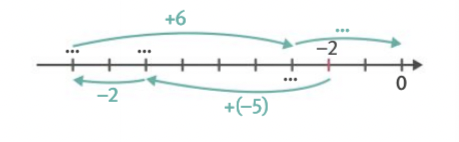
\includegraphics[width = 15 cm]{Exo6}
\newpage
\textbf{Exercice 5} (5,5 points + 2 points)

\begin{figure}[H]\center
\begin{tikzpicture}
\draw[dotted](-5.5,-4.5) grid (7.5,6.5);
\draw[very thick, ->] (-5.5, 0)--(7.5,0);
\draw[very thick, ->] (0,-4.5)--(0,6.5);
\fill (2,-3) circle(.1);
\draw (2,-3) ++ (.25, .25) node {$A$};
\fill (-2,2) circle(.1);
\draw (-2,2) ++ (.25, .25) node {$B$};
\fill (6,4) circle(.1);
\draw (6,4) ++ (.25, .25) node {$C$};
\draw (1,.3) node {$1$};
\draw (.3,1) node {$1$};
\end{tikzpicture}
\end{figure}
1) Indiquer les coordonnées des points $A$, $B$ et $C$. 

2) Placer le point $D$ de coordonnées $(2; 5)$ et le point $E$ de coordonnées $(-3; 2)$. 

3) Placer le point $F$ qui a la même abscisse que $A$ et la même 
ordonnée que $C$. 

4) Placer le point $G$ dont l'abscisse est le tiers de la somme des 
abscisses de $A$, $B$ et $C$, et dont l'ordonnée est le tiers de la 
somme des ordonnées de $A$, $B$ et $C$. 

5) Tracer les droites $(AG)$, $(BG)$ et $(CG)$, et le triangle $ABC$. 

6) Que représentent les droites ainsi tracées pour le triangle $ABC$ ?

\end{document}